%!TEX Program = xelatex
\documentclass[15pt, a4paper]{ctexart}

\usepackage[a4paper, left=1.5cm, right=1.5cm, top=1.5cm, bottom=1.5cm]{geometry}
\usepackage{fancyhdr,pgfplots}
\usepackage{lastpage,caption,siunitx,booktabs} % 用于显示总页数
\usepackage{xcolor}   % 用于颜色
\usepackage{graphicx,wrapfig}
\usepackage{amsmath, amssymb, amsthm}
\usepackage{geometry}
\usepackage{setspace}
\pagestyle{fancy}
\fancyhf{} % 清空默认设置

% 自定义页码格式：左侧显示章节，右侧显示"第X页/共Y页"
\fancyhead[R]{第\thepage 页 / 共\pageref{LastPage}页}
%opening
\title{一种面向果壳航模比赛的无人运输机设计}
\author{陈曦、李卓润、王静雯、陈晓萌、林泽华、许嘉木}

\begin{document}
	
	\maketitle
	
	\begin{abstract}
		本飞行器设计面向果壳航模比赛战略需求，旨在填补低空短途运输领域的运力空缺，提升通用航空基础设施之间的空中联通效率。其主要任务是执行通用航空机场之间的紧急小型货物运输任务，具备良好的起降性能与较高的运行频次适应能力，满足低空经济发展对灵活、高效运输平台的迫切需求。
		
		同时，该飞行器还具备一定的多用途能力，可根据任务改装后执行操场侦察任务，可加装计算机视觉模块(OpenCV)与通用人工智能芯片实现低成本前缘侦察，方便进行对在宽阔地带上课进行"考勤"。通过兼顾民用与校用需求，该飞行器在满足经济发展需要的同时，也具备一定的战略意义。
		
	\end{abstract}
	
	\section{气动布局选型设计}
	\subsection{设计需求与挑战}
	本项目旨在设计一种载重0.3kg的小型固定翼无人机，可满足物资运输等多种应用场景需求。此类无人机面临以下关键技术挑战：
	\begin{enumerate}
		\begin{spacing}{0.8}
			\item 高载重与长航程平衡：在保证有效载荷的同时，实现航程要求，需要优化气动布局与推进系统效率。
			\item 短距起降能力：为适应偏远地区(指怀柔)的简易跑道条件，需具备良好的短距起降(STOL)性能。
		\end{spacing}
	\end{enumerate}
	
	\subsection{总体设计思路}
	综合考虑载重0.3kg的无人机设计需求，以及短距起降能力等特殊要求，在对比分析上单翼布局、常规布局、鸭式布局、双尾撑布局、飞翼布局和三翼面布局等集中主要气动布局方案优缺点后，本项目采用常规布局与单发螺旋桨发动机相结合的设计方案。该设计的主要性能指标为：
	\begin{itemize}
		\begin{spacing}{0.8}
			\item 最大起飞重量：约1.3~kg
			\item 有效载荷：约0.3~kg
			\item 最大飞行高度：100米
			\item 短距起降性能：100米跑道起降能力
			\item 货舱容积：2345~$\rm cm^3$(前舱),388.8~$\rm cm^3$(后舱)
			\item 动力系统：单发固定螺旋桨
		\end{spacing}
	\end{itemize}
	
	\begin{center}
		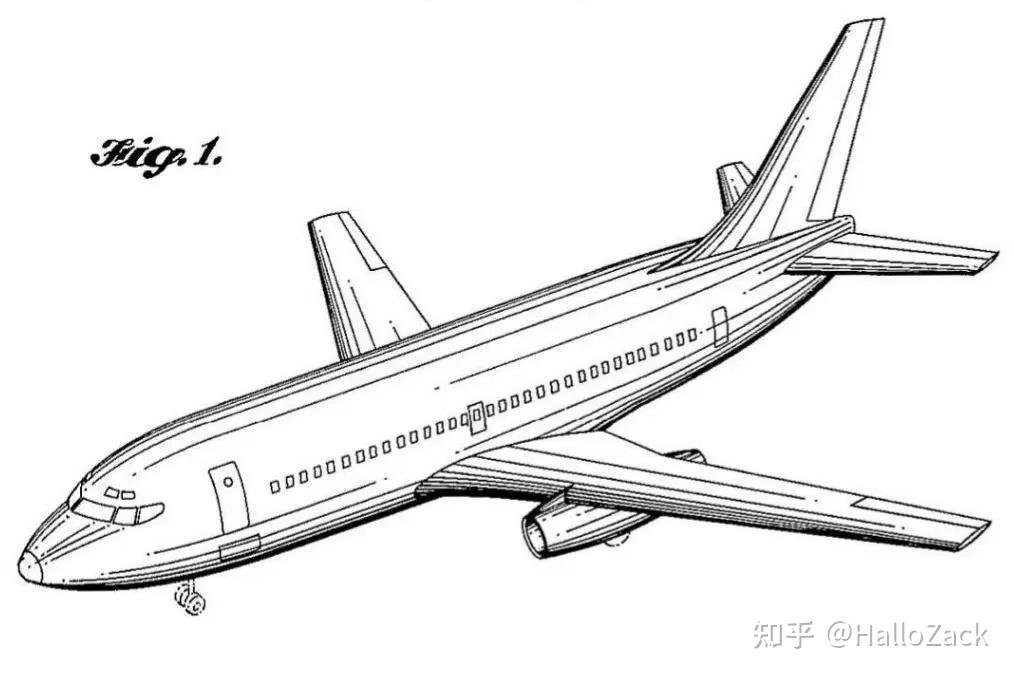
\includegraphics[width=0.5\linewidth]{Boeing737.jpg}
		\captionof{figure}{无人机设计灵感来源}
	\end{center}
	
	\subsection{主要构型参数}
	\begin{center}
		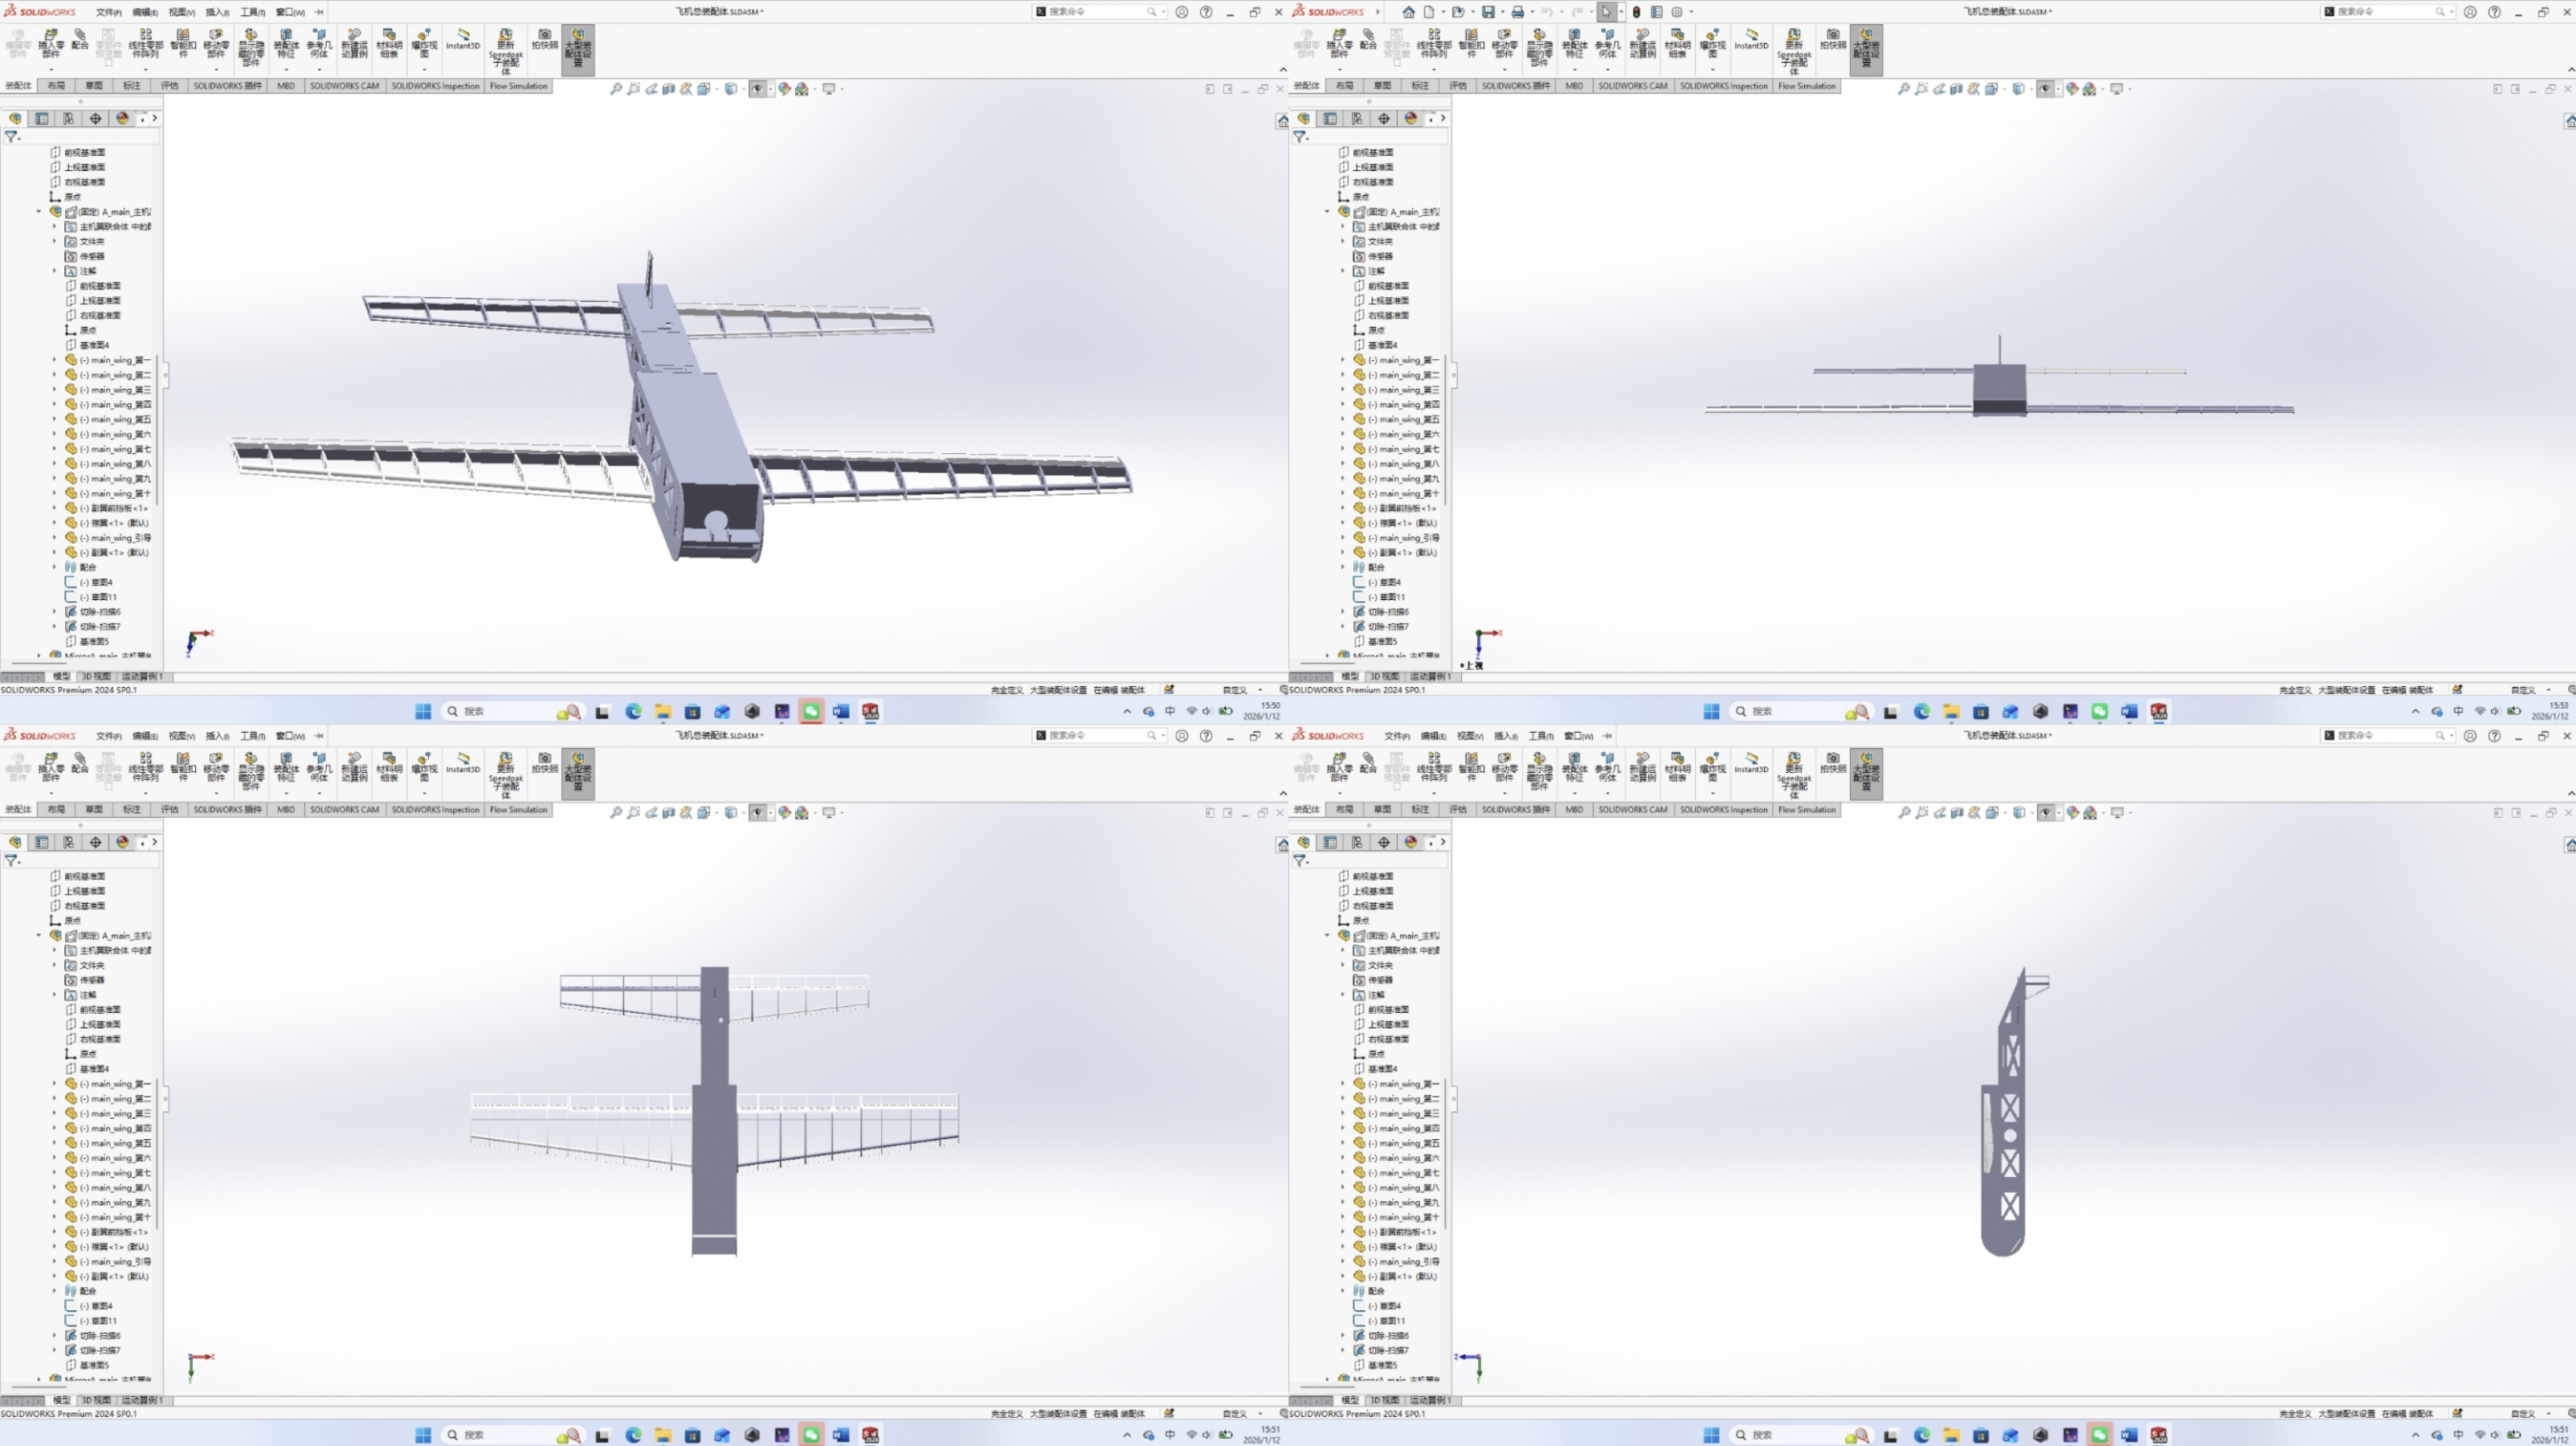
\includegraphics[width=0.7\linewidth]{Tri-graph.jpg}
		\captionof{figure}{飞机三视图}
	\end{center}
	该无人机的主要气动构型参数如下：
	\begin{itemize}
		\begin{spacing}{0.8}
			\item 翼展：1.142~m(包含机身宽度104mm)
			\item 机身长度：0.679~m
			\item 主翼面积：1576.193~cm$^2$
			\item 主翼后掠角：7.61°
			\item 主翼展弦比：8.27
			\item 水平尾翼翼展：0.722~m(包含机身宽度64mm)
			\item 水平尾翼面积: 622.468~cm$^2$
			\item 水平尾翼后掠角：6.87°
			\item 水平尾翼展弦比：8.37
			\item 垂直尾翼翼展(高度)：0.057~m
			\item 垂直尾翼面积：24.453~cm$^2$
			\item 垂直尾翼后掠角：26.6°
			\item 垂直尾翼展弦比：1.33
			\item 主翼-水平尾翼间距(水平)：16.214~cm
			\item 主翼-水平尾翼间距(竖直)：5.0~cm
		\end{spacing}
	\end{itemize}
	
	%补充说明一下，我今天简单地跑了一下X5发现好像这里的C_\mathrm{L,max}取大了，所以我将你下面的缩小为了 C_{L,max}=1.2  一般的C_L = 1.0这应该才是差不多的数据，数据给你调整了一下，你也可以检查一下有无什么问题
	
	\subsection{总体设计参数选择}
	由于飞机为电力驱动，认为其质量不变。当质量为 $m$ 的飞机在高度 $h$ 时，设速度为 $v$，由能量守恒，我们有方程
	\[
	(F-D-R)v=mg\frac{\mathrm dh}{\mathrm dt}+m\frac{\mathrm d}{\mathrm dt}\frac{v^2}{2}
	\]
	其中 $F$ 是动力，$D$ 是气动阻力，$R$是其它阻力。变形得到
	\[
	\frac{F}{mg}=\frac{D+R}{mg}+\frac{1}{v}\frac{\mathrm d}{\mathrm dt}\left(h+\frac{v^2}{2g}\right).
	\]
	现在我们求 $D$。首先，对于升力系数 $C_\mathrm L$，我们有
	\[
	(\mathrm{Lift})=nmg=\frac{1}{2}C_\mathrm L\rho Sv^2\Rightarrow C_\mathrm L=\frac{nmg}{qS},
	\]
	其中 $n$ 为过载，$q=\rho v^2/2$ 为动压，$\rho$ 为空气密度，$S$ 为面积。同时，我们将 $D$ 和 $C_\mathrm L$ 的关系近似为二次函数，并假定其一次项系数为0，也就是
	\[
	D=qS(C_{\mathrm D0}+K_1C_\mathrm L^2)=qS\left(C_{\mathrm D0}+K_1\left(\frac{nmg}{qS}\right)^2\right)
	\]
	代入之前的方程就有
	\[
	\frac{F}{mg}=\frac{1}{mg}\left(qS\left(C_{\mathrm D0}+K_1\left(\frac{nmg}{qS}\right)^2\right)+R\right)+\frac{1}{v}\frac{\mathrm d}{\mathrm dt}\left(h+\frac{v^2}{2g}\right),
	\]
	我们称其为主控方程。
	
	\subsubsection{起飞过程}
	在起飞过程中，$h$ 不变，且认为 $F\gg D+R$ 并略去这两项，就从主控方程得到
	\[
	\frac{F}{mg}=\frac{1}{2vg}\frac{\mathrm d}{\mathrm dt}v^2=\frac{1}{g}\frac{\mathrm dv}{\mathrm dt}=\frac{1}{g}\frac{\mathrm dv}{\mathrm dx}v.
	\]
	解这个微分方程，并代入初始条件和终末条件 $x=x_{\rm T.O.}$ 得到
	\[
	x_{\mathrm{T.O.}}=\frac{mv_{\mathrm{T.O.}}^2}{2F}.
	\]
	仿照书本定义起飞安全速度系数 $k_{\mathrm{T.O.}}=v_\mathrm {T.O.}/v_\mathrm S$，其中下标S表示失速。同时由 $mg=C_\mathrm L\rho Sv_\mathrm S^2/2$ 解出 $v_\mathrm S=\sqrt{2mg/(\rho SC_\mathrm {L,max})}$。再代入上面的方程，就得到
	\[
	v_\mathrm {T.O.}=k_{\mathrm{T.O.}}\sqrt{\frac{2mg}{\rho SC_\mathrm {L,max}}}
	\]
	\[
	x_{\mathrm{T.O.}}=\frac{m^2k_{\mathrm{T.O.}}^2g}{F\rho SC_\mathrm {L,max}}
	\]
	和起飞距离约束方程
	\[
	\frac{F}{mg}=\frac{k_{T.O.}^2}{x_\mathrm {T.O.}\rho C_\mathrm{L,max}}\frac{m}{S}
	\]
	在这里取 $(g,\,k_\mathrm{T.O.},\,x_\mathrm{T.O.},\,\rho,\,C_{\mathrm{L,max}})=(9.8,\,1.2,\,100,\,1.213,\,1.2)$ 并采用国际单位制，就可以计算得起飞距离约束方程
	\[
	\frac{F}{mg}=\frac{k_{T.O.}^2}{x_\mathrm {T.O.}\rho C_\mathrm{L,max}}\frac{m}{S}\approx0.009\,89\,(\mathrm{m^2/kg})\,\frac{m}{S}
	\]
	%Note: 这里计算出来F只需要0.56N，我觉得有疑问，但也不是特别有疑问。但是其它的两项数据十分正常。
	
	\subsubsection{着陆过程}
	此时有 $F\ll R+D\approx \mu mg$，由牛顿第二定律
	\[
	\mu mg=m\frac{\mathrm d^2x}{\mathrm dt^2}\Rightarrow x_\mathrm {LGR}=\frac{v_\mathrm{T.D.}^2}{2\mu g}
	\]
	其中 $x_\mathrm{LGR}$ 是滑跑距离，$v_\mathrm{T.D.}$ 是接地速度。定义着陆接地安全速度系数 $k_\mathrm{T.D.}=v_\mathrm{T.D.}/v_\mathrm S$，就可以得到
	\[
	x_\mathrm{LGR}=\frac{k_\mathrm{T.D.}^2}{2\mu g}\frac{2mg}{\rho SC_\mathrm {L,max}}=\frac{k_\mathrm{T.D.}^2m}{\mu\rho SC_\mathrm{L,max}}
	\]
	以及滑跑距离约束方程
	\[
	\frac{m}{S}=\frac{\mu x_\mathrm{LGR}\rho C_\mathrm{L,max}}{k_\mathrm{T.D.}^2}
	\]
	取$(x_\mathrm{LGR},\,k_\mathrm{T.D.},\,\mu,\,\rho,\,C_{\mathrm{L,max}})=(100,\,1.3,\,0.2,\,1.213,\,1.2)$ 并采用国际单位制计算得到滑跑距离约束方程
	\[
	\frac{m}{S}=\frac{\mu x_\mathrm{LGR}\rho C_\mathrm{L,max}}{k_\mathrm{T.D.}^2}\approx 17.226\,\mathrm{kg/m^2}
	\]
	
	\subsubsection{极速}
	当飞机达到极速时，认为 $h$ 不变，$v$ 不变，$R\approx 0$，无过载，则主控方程变为
	\[
	\frac{F}{mg}=\frac{1}{mg}qS\left(C_{\mathrm D0}+K_1\left(\frac{mg}{qS}\right)^2\right)
	\]
	此时选取 $C_\mathrm{L,min}=C_\mathrm{D0}$ 和 $K_1=1/(\pi Ae)$，其中 $A$ 为展弦比，$e$ 为 Ostwald 系数，根据如下经验公式确定
	\[
	e=4.61(1-0.045A^{0.68})(\cos \varLambda)^{0.15}-3.1.
	\]
	其中 $\varLambda$ 是机翼后掠角。则主控方程又变为
	\[
	\frac{F}{mg}=C_\mathrm{L,min}\frac{\rho v^2}{2g}\left(\frac{m}{S}\right)^{-1}+\frac{1}{\pi Ae}\frac{2g}{\rho v^2}\left(\frac{m}{S}\right)
	\]
	取 $(A,\,\varLambda,\,C_\mathrm{L,min},\,\rho,\,v,\,g)=(8.27,\,7.61^\circ,\,0.5,\,1.213,\,12,\,9.8)$ 并使用国际单位制，计算得到 $e\approx 0.632\,439\,8$ 和约束方程
	\[
	\frac{F}{mg}=C_\mathrm{L,min}\frac{\rho v^2}{2g}\left(\frac{m}{S}\right)^{-1}+\frac{1}{\pi Ae}\frac{2g}{\rho v^2}\left(\frac{m}{S}\right)\approx 4.456\,(\mathrm{kg/m^2})\,\left(\frac{m}{S}\right)^{-1}+0.006\,83\,(\mathrm{m^2/kg})\,\left(\frac{m}{S}\right).
	\]
	
	作出三个约束方程的图形(如图3，其中纵轴表示 $F/(mg)$，横轴表示 $m/S$)
	\begin{center}
		\begin{tikzpicture}
			\begin{axis}[
				width=0.6\textwidth,
				height=0.5\textwidth,
				xlabel={$m/S$ (kg/m$^2$)},
				ylabel={$F/(mg)$},
				xmin=0, xmax=120,
				ymin=0, ymax=2,
				grid=both,
				grid style={line width=0.1pt, draw=gray!30},
				major grid style={line width=0.2pt, draw=gray!50},
				axis lines=left,
				legend style={at={(0.98,0.98)}, anchor=north east, cells={anchor=west}},
				title={飞机设计约束条件示意图},
				xtick={0,20,40,60,80,100,120},
				extra x ticks={17.226},
				extra x tick labels={17.23},
				extra x tick style={grid style={red, dashed}, tick label style={red}},
				ytick={0,0.5,1.0,1.5,2.0},
				scaled y ticks=false,
				%会用吗
				y tick label style={/pgf/number format/fixed},
				x tick label style={/pgf/number format/fixed},
				]
				
				% 起飞约束曲线: F/(mg) = 0.00989 * (m/S)
				\addplot[domain=0:120, samples=200, thick, blue, line width=1.5pt] 
				{0.00989*x};
				\addlegendentry{起飞距离约束: $F/(mg) = 0.00989(m/S)$};
				
				% 着陆约束垂直线: m/S = 17.226
				\addplot[domain=0:2, samples=2, thick, red, dashed, line width=1.5pt] 
				coordinates {(17.226,0) (17.226,2)};
				\addlegendentry{着陆滑跑距离约束: $m/S = 17.23$};
				
				% 极速约束曲线: F/(mg) = 4.456*(m/S)^{-1} + 0.00683*(m/S)
				\addplot[domain=1:120, samples=200, thick, green, line width=1.5pt] 
				{4.456/x + 0.00683*x};
				\addlegendentry{极速约束: $F/(mg) = 4.456(m/S)^{-1} + 0.00683(m/S)$};
				
				% 计算极速约束的最小值点
				% 对 y = 4.456/x + 0.00683x 求导:
				% y' = -4.456/x² + 0.00683 = 0
				% x_min = sqrt(4.456/0.00683) ≈ sqrt(1305.42) ≈ 
				\pgfmathsetmacro{\xmin}{sqrt(4.456/0.00683)}
				\pgfmathsetmacro{\ymin}{4.456/\xmin + 0.00683*\xmin}
				
				% 标注极速约束最小值点
				\node[draw=black, fill=white, inner sep=2pt, circle, pin={[pin distance=8mm]-40:{最小值点 $(\approx 25.54, \approx 0.349)$}}] 
				at (axis cs:\xmin,\ymin) {};
				
				% 标注起飞约束和极速约束的交点
				% 解方程: 0.00989x = 4.456/x + 0.00683x
				% 0.00989x - 0.00683x = 4.456/x
				% 0.00306x = 4.456/x
				% 0.00306x² = 4.456
				% x² = 4.456/0.00306 ≈ 2912.42
				% x ≈ 38.16
				% y ≈ 0.00989*38.16 ≈ 0.377
				\pgfmathsetmacro{\xintersect}{sqrt(4.456/0.00306)}
				\pgfmathsetmacro{\yintersect}{0.00989*\xintersect}
				
				\node[draw=black, fill=white, inner sep=2pt, circle, pin={[pin distance=10mm]45:{交点 $(\approx 38.16, \approx 0.377)$}}] 
				at (axis cs:\xintersect,\yintersect) {};
				
				% 标注着陆约束与起飞约束的交点
				\node[draw=black, fill=white, inner sep=2pt, rectangle, pin={[pin distance=8mm]+85:{交点 $(17.23, 0.170)$}}] 
				at (axis cs:17.226,0.1704) {};
				
				% 添加坐标轴标注
				\node[red] at (axis cs:17.226,2.05) {$m/S = 17.23$};
				
				% 显示可行区域
				\node at (axis cs:12,1.3) {可行区域};
				
				% 添加参考线
				\addplot[domain=0:120, samples=2, black!50, dashed, line width=0.5pt] 
				{0.5};
				\node[black!50] at (axis cs:80,0.52) {$F/(mg)=0.5$};
				
				\addplot[domain=0:120, samples=2, black!50, dashed, line width=0.5pt] 
				{1.0};
				\node[black!50] at (axis cs:80,1.02) {$F/(mg)=1.0$};
				
			\end{axis}
		\end{tikzpicture}
		
		\captionof{figure}{飞机设计约束条件示意图：起飞距离约束（蓝色实线）、着陆滑跑距离约束（红色虚线）和极速约束（绿色实线）。横坐标为翼载 $m/S$，纵坐标为推力重量比 $F/(mg)$。着陆约束表现为一条垂直直线，对应 $m/S = 17.226\ \mathrm{kg/m^2}$。点 $A$ 表示起飞约束与着陆约束的交点。}
		\label{fig:constraints}
	\end{center}
	
	本飞机取值：$(m/S)=1.3\,\mathrm{kg}/0.22\,\mathrm m^2\approx 5.909\,\mathrm{kg/m^2}$，代入图形得最小推重比为0.794，此处我们取0.8制作。
	
	%下面是我自己对机翼的论述，不用修改
	\subsection{无人机各部件设计}
	\subsubsection{主机翼与水平尾翼几何参数设计}
	已知：最大起飞重量$m_0=1.3\,\mathrm{kg}$，机翼面积$S=2,198.661\,\mathrm{cm^2}$，主机翼展长$I_{\text{主机翼}}=1.142\,\mathrm{m}$，后掠角$Λ=7.61°$，巡航高度暂定$100\,\mathrm{m}$，机翼分主翼和水平尾翼、垂直尾翼三部分，其中产生升力的机翼中，主翼占$71.68\%$升力面积，水平尾翼占$28.32\%$升力面积
	\begin{enumerate}
		\item[(1)主机翼].\\
		展弦比：\[A=\frac{I_{\text{主机翼}}^2}{71.68\% S}=8.27\]
		飞机构型采用后掠机翼，当梢根比为0.4-0.5左右时，机翼产生的诱导阻力是最小的，因此取梢根比为 $\lambda_{\text{主机翼}} = 0.628$，
		翼根弦长为 $C_{root}=186.5\,\mathrm{mm}$，
		翼尖弦长为 $C_{tip}=\lambda_{\text{主机翼}} C_{root}=117.2\,\mathrm{mm}$
		
		由于采用简单梯形机翼，利用几何平均法得到飞机的平均气动弦长
		\[\bar{c}=0.5\times (C_{root}+C_{tip})=161.85\,\mathrm{mm}\]
		平均气动弦距机身轴线的距离为
		\[\bar{Y}=\frac{1}{2}I_{\text{主机翼}}=571\,\mathrm{mm}\]
		\item[(2)水平尾翼].\\
		水平尾翼的参数设计与主翼类似，取水平尾翼翼展为$329\,\mathrm{mm}$\\
		展弦比：
		\[A=\frac{I_{\text{水平尾翼}}^2}{28.32\%S}=8.37\]
		水平尾翼构型采用后掠机翼，当梢根比为0.4-0.5左右时，水平尾翼产生的诱导阻力是最小的，因此取梢根比为 $\lambda_{\text{水平尾翼}}=0.654$，    翼根弦长为 $C_{root}=114.4\,\mathrm{mm}$
		翼梢弦长为 $C_{tip}=\lambda_{\text{水平尾翼}} C_{root}=74.8\,\mathrm{mm}$
		
		由于采用简单梯形机翼，利用几何平均法得到飞机的平均气动弦长
		\[\bar{c}=0.5\times (C_{root}+C_{tip})=94.6\,\mathrm{mm}\]
		平均气动弦距机身轴线的距离为
		\[\bar{Y}=\frac{1}{2}I_{\text{水平尾翼}}=180.5\,\mathrm{mm}\]
		而对于拉力式螺旋桨飞机，设计飞机重心在飞机主翼的前25\%平均气动弦长附近,所以尾力臂约为
		\[L\approx 280\,\mathrm{mm}\]
		带入计算水平尾翼的尾容量为
		\[\text{尾容量}=\frac{\text{平尾面积}\times\text{尾力臂}}{\text{主翼面积}\times\text{平均气动弦长}}=\frac{62246.8\times 280}{94.6\times 157619.3}=1.17\]
	\end{enumerate}
	从而得到主机翼与水平尾翼重要几何参数如下
	\begin{table}[h!]
		\centering
		\caption{主机翼与水平尾翼重要几何参数}
		\begin{tabular}{|c|c|c|}
			\hline
			\textbf{参数} & \textbf{主机翼} & \textbf{水平尾翼} \\ \hline
			机翼面积(产生升力的，单位：$\,\mathrm{cm^2}$) & 1576.193 & 622.468 \\ \hline
			稍根比 & 0.628 &  0.654 \\ \hline
			展弦比 & 8.27 & 8.37 \\ \hline
			后掠角 & 7.61$^o$ & 6.87$^o$ \\ \hline
			展长(包含相应位置机厢宽度) & 1.142 米 (含宽度 104mm) & 0.722 米 (含宽度 64mm) \\ \hline
			翼根弦长 & 186.5mm & 114.4mm\\ \hline
			翼梢弦长 & 117.2 mm & 74.8mm \\ \hline
			平均气动弦长 & 139.875mm & 85.8mm \\ \hline
			平均气动弦距 & 571mm & 180.5mm \\ \hline
			安装角 & 1$^o$ & - \\ \hline
			扭转角($\varepsilon_{root}$) & 2$^o$ & 2$^o$ \\ \hline
			扭转角($\varepsilon_{tip}$) & -2$^o$ & -2$^o$ \\ \hline
			上反角 & -3$^o$ & -3$^o$ \\ 
			\hline
		\end{tabular}
	\end{table}
	\subsubsection{主机翼安装角，扭转角，上反角的选择}
	\begin{enumerate}
		\item[(1)安装角$i_w$] :\\
		恰当的安装角可以使机翼在选定的迎角下，机身迎角刚好处于使机身阻力最小的条件。安装角的最终确定要由吹风实验决定，对初始设计工作，它可以由统计数据决定，并在后面的气动计算中加以检验。暂取
		\[i_w=1^\circ\]
		\item[(2)扭转角$\varepsilon$] :\\
		一定的扭转可以防止翼尖失速并修正机翼的升力分布，使其接近理想的椭圆分布。一般机翼扭转角在0~5之间。在初试设计阶段，暂不考虑气动扭转，气动扭转需要结合吹风实验才能确定。此处，采用统计数值来确定，取扭转角为：
		\[\varepsilon_{root}=2°,\varepsilon_{tip}=-2°\]
		\item[(3)上反角$\Gamma_w$] :\\
		反角可以使飞机受到扰动而倾斜时自动改平，即增加了飞机航向静稳定性。上反角的最终确定十分复杂，暂时由统计结果确定,取：
		\[\Gamma_w=-3^\circ\]
	\end{enumerate}
	
	\subsubsection{副翼襟翼的计算}
	\begin{enumerate}
		\item[(1)襟翼]:\\
		采用后缘简单襟翼，从翼根开始，延伸到55.8\%展长处，其弦长也取为机翼翼梢弦长的23.6\%.
		\[C_a = 44\,\mathrm{mm}\]
		后缘简单襟翼偏转角设计：
		\begin{itemize}
			\begin{spacing}{0.8}
				\item 起飞状态：下偏$10^\circ-15^\circ$（此处取$12^\circ$）
				\item 着陆状态：下偏$30^\circ-40^\circ$（此处取$35^\circ$）
				\item 最大下偏：$40^\circ$
			\end{spacing}
		\end{itemize}
		
		襟翼对升力系数的增量(简单估计)：
		\[\Delta C_{L\text{max}} = \Delta C_{L\text{max flap}} \times \frac{S_{\text{flap}}}{S} \times \cos(\Lambda)\]
		
		简单襟翼$\Delta C_{L\text{max flap}} = 0.9$，襟翼面积占比55.8\%：
		\[\Delta C_{L\text{max}} = 0.9 \times 0.558 \times \cos(7.61^\circ) = 0.498\]
		
		着陆襟翼偏转$35^\circ$时，最大升力系数从1.2增至1.698，显著改善着陆性能。
		\item[(2)副翼]：\\
		副翼的面积一般取为机翼面积的5\%-7\%，此处取$S_a=7.16\% S$
		\[S_a=157.5\,\mathrm{cm^2}\]
		副翼的相对弦长约为机翼弦长的20\%-25\%,此处取$C_a=23.6\%C_{\text{靠近翅根的那一端的弦长}}$
		\[C_a=35\,\mathrm{mm}\]
		副翼用于滚转控制。副翼偏转角设计：
		\begin{itemize}
			\begin{spacing}{0.8}
				\item 正常滚转：上下各$10^\circ$
				\item 快速滚转：上下各$20^\circ$
				\item 最大偏转角：$\pm 25^\circ$
			\end{spacing}
		\end{itemize}
		副翼铰链力矩计算（单侧副翼）：
		\[M_{ha} = q \times S_{a\text{单}} \times C_a \times C_{h\delta_a} \times \delta_a\]
		单侧副翼面积$S_{a\text{单}} = 157.5/2 = 78.75\,\text{cm}^2 = 0.007875\,\text{m}^2$，
		$C_a = 0.035\,\text{m}$，
		$C_{h\delta_a} = -0.35$，
		$\delta_a = 15^\circ = 0.262\,\text{rad}$：
		\[M_{ha} = 136.5 \times 0.007875 \times 0.035 \times (-0.35) \times 0.262 = -0.00345\,\text{N·m}\]
		所需舵机扭矩：
		\[T_{a\text{req}} = \frac{3.0 \times 0.00345}{0.8} = 0.0129\,\text{N·m}\]
		选择标准舵机：扭矩0.2 N·m，满足要求。
		\begin{center}
			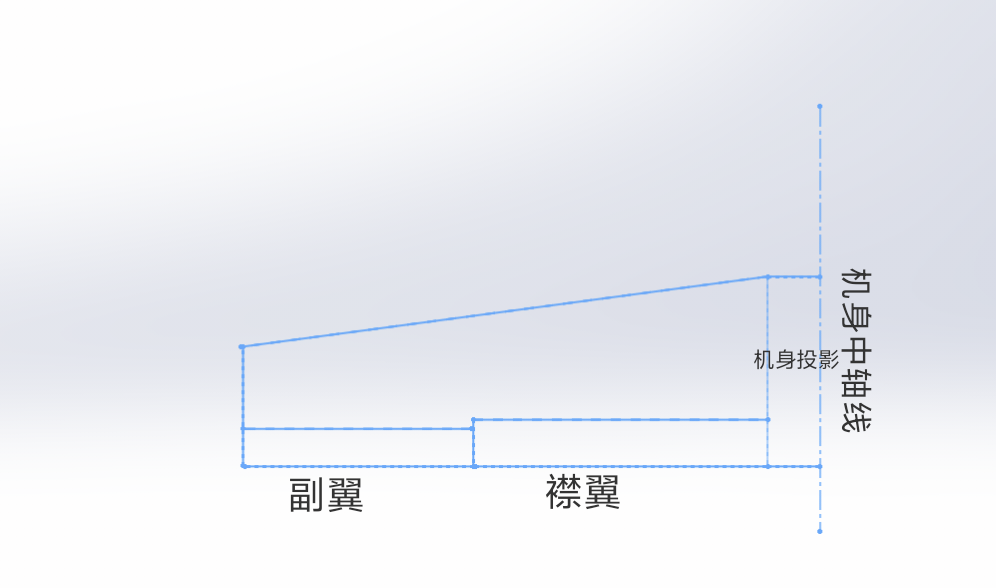
\includegraphics[width=0.5\columnwidth]{main_wing_combination.png}
			\captionof{figure}{襟翼副翼布置图}
		\end{center}
		
	\end{enumerate}
	\subsubsection{升降舵的计算}
	升降舵位于水平尾翼后缘，用于控制飞机的俯仰运动。根据规范，升降舵面积一般取水平尾翼面积的25\%-40\%，此处取：$36.998\%S$
	\[S_e=36.998\%S=230.3\,\mathrm{cm^2}\]
	升降舵相对弦长取水平尾翼弦长的30\%-40\%，此处取：$30.6\%$相对翼根处弦长
	\[C_e=35\,\mathrm{mm}\]
	\begin{enumerate}
		\item[(1) 偏转角度设计]：\
		升降舵偏转角根据飞行状态确定，小型无人机通常采用：
		\begin{itemize}
			\begin{spacing}{0.8}
				\item 起飞阶段：上偏$+15^\circ$，下偏$-20^\circ$
				\item 巡航阶段：上偏$+10^\circ$，下偏$-15^\circ$
				\item 着陆阶段：上偏$+20^\circ$，下偏$-25^\circ$
			\end{spacing}
		\end{itemize}
		最大偏转角限制为$\pm 30^\circ$。
		\item[(2) 操纵力计算]：\\
		首先计算升降舵的铰链力矩。在巡航状态下，取巡航速度$V=15\,\text{m/s}$，空气密度$\rho=1.213\,\text{kg/m}^3$：
		\[q = \frac{1}{2}\rho V^2 = \frac{1}{2} \times 1.213 \times 15^2 = 136.5\,\text{Pa}\]
		升降舵铰链力矩公式：
		\[M_h = q \times S_e \times C_e \times C_{h\delta} \times \delta_e\]
		对于无补偿的升降舵，铰链力矩系数导数$C_{h\delta} \approx -0.6$。采用30\%的轴式补偿后，$C_{h\delta} \approx -0.3$。
		以最大下偏角$\delta_e = -20^\circ = -0.349\,\text{rad}$为例：
		\[M_h = 136.5 \times 0.02303 \times 0.0263 \times (-0.3) \times (-0.349) = 0.00277\,\text{N·m}\]    
		考虑安全系数3.0和传动效率0.8，所需舵机扭矩：
		\[T_{\text{req}} = \frac{3.0 \times 0.00277}{0.8} = 0.0104\,\text{N·m}\]
		选择标准舵机：扭矩0.2 N·m，满足要求。
		\item[(3) 配平能力验证]: \\
		验证升降舵在重心范围内的配平能力。飞机重心范围：25\%-35\% MAC。
		
		水平尾翼升力系数增量：
		\[\Delta C_{L_t} = C_{L\alpha_t} \cdot \eta_t \cdot \frac{S_t}{S} \cdot \tau_e \cdot \delta_e\]
		
		其中：$C_{L\alpha_t} = 2\pi/\text{rad} = 0.11/\text{deg}$（水平尾翼升力线斜率），
		$\eta_t = 0.9$（尾翼效率系数），
		$S_t/S = 622.468/2198.661 = 0.283$，
		$\tau_e = 0.8$（升降舵效率因子）。
		
		在重心后限（35\% MAC），需配平俯仰力矩。计算所需升降舵偏角：
		\[\delta_{e\text{trim}} = \frac{C_{m0} + C_{m\alpha}\alpha}{C_{m\delta_e}} \approx \frac{0.02 + 0.1\alpha}{0.02} = 1 + 5\alpha\]
		
		在巡航迎角$\alpha=4^\circ$时：
		\[\delta_{e\text{trim}} = 1 + 5\times4 = 21^\circ\]
		
		在升降舵偏转范围$(-25^\circ, +20^\circ)$内，可以满足配平要求。
	\end{enumerate}
	\subsubsection{垂直尾翼设计}
	本飞机同时拥有水平尾翼与垂直尾翼。因此接下来设计垂直尾翼，垂直尾翼设计为同样具有后掠角的梯形翼。当梢根比为0.4-0.5左右时，机翼产生的诱导阻力是最小的，因此取梢根比为
	\[\lambda_{\text{垂直尾翼}} = 0.5\]
	翼根弦长：\[C_{root}=57.2\,\mathrm{mm}\]
	翼梢弦长：\[C_{tip}=28.6 \,\mathrm{mm}\]
	展弦比：\[A=\frac{I_{\text{垂直尾翼}^2}}{S_{\text{垂直尾翼}}}=1.33\]
	同样采用与之前计算水平尾翼尾容量相同的方法，取重心在主机翼0.25MAC处，估计尾力臂为
	\[L\approx 340\,\mathrm{mm}\]
	所以计算尾容量有
	\[\text{尾容量}=\frac{\text{平尾面积}\times\text{尾力臂}}{\text{主翼面积}\times\text{平均气动弦长}}=\frac{2445.3\times 340}{64.35\times 157619.3}=0.82\]
	
	\subsubsection{方向舵的设计}
	方向舵位于垂直尾翼后缘，用于控制飞机的偏航运动。此处取方向舵面积为：
	\[S_r = 11.4\ \text{cm}^2\]
	方向舵相对弦长取垂直尾翼翼根弦长的30\%-40\%，此处取35.08\%：
	\[C_r = 20\ \text{mm}\]
	
	\begin{enumerate}
		\item[(1) 偏转角度设计]：\\
		方向舵偏转角根据飞行状态确定，小型无人机通常采用：
		\begin{itemize}
			\begin{spacing}{0.8}
				\item 正常转弯：左右各$15^\circ$
				\item 大角度转弯/侧风修正：左右各$25^\circ$
				\item 最大偏转角：$\pm 30^\circ$
			\end{spacing}
		\end{itemize}
		
		\item[(2) 操纵力计算]：\\
		计算方向舵的铰链力矩。在巡航状态下，取巡航速度$V=15\,\text{m/s}$，空气密度$\rho=1.213\,\text{kg/m}^3$：
		\[q = \frac{1}{2}\rho V^2 = 136.5\ \text{Pa}\]
		
		方向舵铰链力矩公式：
		\[M_{hr} = q \times S_r \times C_r \times C_{h\delta_r} \times \delta_r\]
		
		对于无补偿的方向舵，铰链力矩系数导数$C_{h\delta_r} \approx -0.6$。采用30\%的轴式补偿后，$C_{h\delta_r} \approx -0.3$。
		
		以最大偏转角$\delta_r = 25^\circ = 0.436\text{rad}$为例：
		\[M_{hr} = 136.5 \times 0.00114 \times 0.02 \times (-0.3) \times 0.436 = -0.00041\ \text{N·m}\]
		
		考虑安全系数3.0和传动效率0.8，所需舵机扭矩：
		\[T_{r\text{req}} = \frac{3.0 \times 0.00041}{0.8} = 0.00154\ \text{N·m}\]
		
		选择标准舵机：扭矩0.2 N·m，完全满足要求。
		
		\item[(3) 偏航控制能力验证]：\\
		验证方向舵在侧风条件下的控制能力。飞机设计最大侧风起降速度为$5\ \text{m/s}$。
		
		侧滑角产生的偏航力矩：
		\[C_{n\beta} = -C_{L\alpha_v} \cdot \eta_v \cdot \frac{S_v}{S} \cdot \frac{l_v}{b} \cdot \left(1 + \frac{\partial\sigma}{\partial\beta}\right)\]
		
		其中：$C_{L\alpha_v} = 0.11/\text{deg}$（垂直尾翼升力线斜率），
		$\eta_v = 0.85$（垂尾效率系数），
		$S_v/S = 0.0111$，
		$l_v = 0.34\ \text{m}$（垂尾力臂），
		$b = 1.142\ \text{m}$（翼展），
		$\partial\sigma/\partial\beta = 0.2$（侧洗因子）。
		
		计算得：$C_{n\beta} \approx -0.0012/\text{deg}$
		
		在5 m/s侧风、15 m/s飞行速度下，侧滑角$\beta \approx 18.4^\circ$，产生的偏航力矩系数：
		\[C_n = C_{n\beta} \cdot \beta = -0.0012 \times 18.4 = -0.0221\]
		
		方向舵偏航力矩系数导数：
		\[C_{n\delta_r} = -C_{L\alpha_v} \cdot \eta_v \cdot \frac{S_r}{S} \cdot \frac{l_v}{b} \cdot \tau_r \approx -0.0008/\text{deg}\]
		
		所需方向舵偏角：
		\[\delta_{r\text{req}} = \frac{C_n}{C_{n\delta_r}} = \frac{-0.0221}{-0.0008} = 27.6^\circ\]
		
		在方向舵最大偏转角$\pm 30^\circ$范围内，能够满足侧风修正需求。
	\end{enumerate}
	
	\subsubsection{机身的设计}
	机身主要分为四段。第一段为机头，长约50 mm，第二段为主机舱，长约350 mm，第三段为后机舱，长约135 mm，第四段为尾翼连接段，长约140 mm。考虑隔板厚度为2 mm，可以控制全机长度在700 mm以内。
	
	机头为半圆形，中间留电机位置，且于上下空位设置风挡。风挡尺寸 $42.5\,\mathrm{mm}\times 100\,\mathrm{mm}$，电机支撑板尺寸 $40\,\mathrm{mm}\times 100\,\mathrm{mm}$，中间有宽度20 mm 的槽供固定电机。
	
	机头与主机舱之间用尺寸为102 mm × 100 mm 的挡板连接，挡板中间开直径为30 mm 的孔，便于走线连接电机。此后是主机舱，有效载荷空间(暂不考虑电机等元器件之占用)为348 mm × 100 mm × 66mm，载荷空间下方为主机翼连接处，主机翼前端距离飞机机头前端之距离大致于 [180.85 mm, 228.49 mm] 区间内可调，且其安装角可调，具体操作方式为橡皮泥填充机翼连接件与机身孔隙。此段高度(包含有效载荷空间之高度与)
	
	主机舱后置尺寸为104 mm × 102 mm 的挡板，用以连接后机舱。后机舱有效载荷空间为135 mm × 60 mm × 48 mm，此段高度为62 mm。后机舱之后用尺寸为60 mm × 60 mm 的挡板分隔它与尾翼连接段。尾翼连接段不封闭，仅存在四面。水平尾翼与侧面连接，垂直尾翼与上表面连接。
	
	机头与主机舱的侧板、后机舱与尾翼连接段的侧板分别作一体化处理。所有使用的板材厚度统一为 $2\,\mathrm{mm}$，上述测量值或因是否计入板材厚度而产生差异。具体细节亦可参考模型内容。
	
	\subsubsection{起落架的设计}
	无人机预计采用前三点式起落架，固定不可收放，并锁死前轮方向。处于结构和连接的考虑，前后起落架均连接于主机舱的底部。先确定起飞预计的攻角。根据飞机模型的几何形状，出于不磨损后置机舱的需要，我们确定无后置配重且主起落架不造成影响时攻角 $\phi$ 满足
	\[
	\phi<\min\left\{\arctan\frac{40}{135},\,\arctan\frac{60}{140}\right\}=\arctan\frac{8}{27}\approx 16.504^\circ. 
	\]
	
	出于减小尺寸和结构稳定性的考量，确定起落架与地面接触点和侧板最低点高度差 $\Delta h_\mathrm G$ 和后起落架距离主舱后缘距离 $x_\mathrm{rear}$ 满足
	\[
	\Delta h_\mathrm G=50\,\mathrm{mm},\,\arctan\frac{\Delta h_\mathrm G}{x_\mathrm{rear}}\geq \arctan\frac{8}{27}\Rightarrow x_\mathrm{rear}\leq 168.75\,\mathrm{mm}.
	\]
	不妨确定 $x_\mathrm{rear}=10\,\mathrm {mm}$，此时主起落架对 $\phi$ 的取值造成影响。此时结构允许的起飞最大角度为 $\phi=\arctan [(100+50)/(0+135+140)]\approx 28.610^\circ$。下考虑前主轮距。假定飞机重心在靠机头0.35 m的位置，那么此时重心与主轮的水平距离为40 mm。考虑到一般飞机前轮受力最好为总重的 $0.08-0.15$ 倍，那么可以取前轮和机头的水平距离为70 mm，此时前轮水平方向距离重心280 mm，就有这一比例为 $40/(280+40)=0.125$，满足要求。此时前主轮距为320 mm。
	
	设主轮间距为 $2d_\mathrm G$，设重心的几何高度为距离地面 70 mm，由简单的立体几何知使得飞机在地面绕前起落架和某侧主轮形成的连线侧翻的临界侧倾角度 
	\[
	\theta_\mathrm{crit}=\arctan \left(\frac{4d_\mathrm G}{\sqrt{320^2+d_\mathrm G^2}}\right)
	\]
	
	命令 $\theta_\mathrm{crit}\geq 45^\circ$，近似得到 $d_\mathrm G\geq 82.624\,\mathrm{mm}$ 则可以取 $d_\mathrm G=85\,\mathrm {mm}$，主起落架轮距为 $170\,\mathrm{mm}$，此时 $\theta_\mathrm{crit}\approx 45.760^\circ$。我们不设置停机角。
	
	值得提及的是，由于跑道可能存在直径为3 mm左右的凸起，需要起落架轮减少使用硬质材料且半径最好超过10 mm。
	
	%啊真的写不动了，交给白天的自己罢，甚至还要先算重心才能确定前主轮距。
	%我估计的重心在主机翼的前1/4平均气动弦长处，你看你觉得是要计算一下还是怎么样
	
	
	
	%剩下的不多，cx巨佬应该可以手拿把掐。我写的这段也给出了求起飞、着陆跑道长度和起飞速度的式子（其中起飞速度的那个式子是基于我们模型里测量的几何参数，而这一段计算是通过估计确定几何参数，有因果倒置之嫌，不应该出现在这一段。但是我都算完了，结果就摆在那里吧，最终稿的这一段计算应该删去那个结果，我只是想着如果需要用到那就不白算）
	%给你移上去了
	\subsubsection{机翼翼型的选择}
	由总体参数可得$C_{Lmax}=1.2$(机翼翼型的$C_{Lmax}=1.6$)，最大升阻比$K_{max}=14$，巡航高度$100m$，巡航速度$15m/s$。得到雷诺数约为190 016。下面利用软件profili计算几种典型大升力翼型的特性曲线。
	
	首先考虑主翼和鸭翼的翼型。典型大升力翼型有Clark Y，NACA 4位数字和5位数字翼型，因此备选Clark Y、NACA 23016，NACA4412，NACA2415四种翼型。分别绘制五种翼型的极曲线、升阻力系数与攻角关系图、升阻比/俯仰力矩与攻角关系图如下：
	\begin{center}
		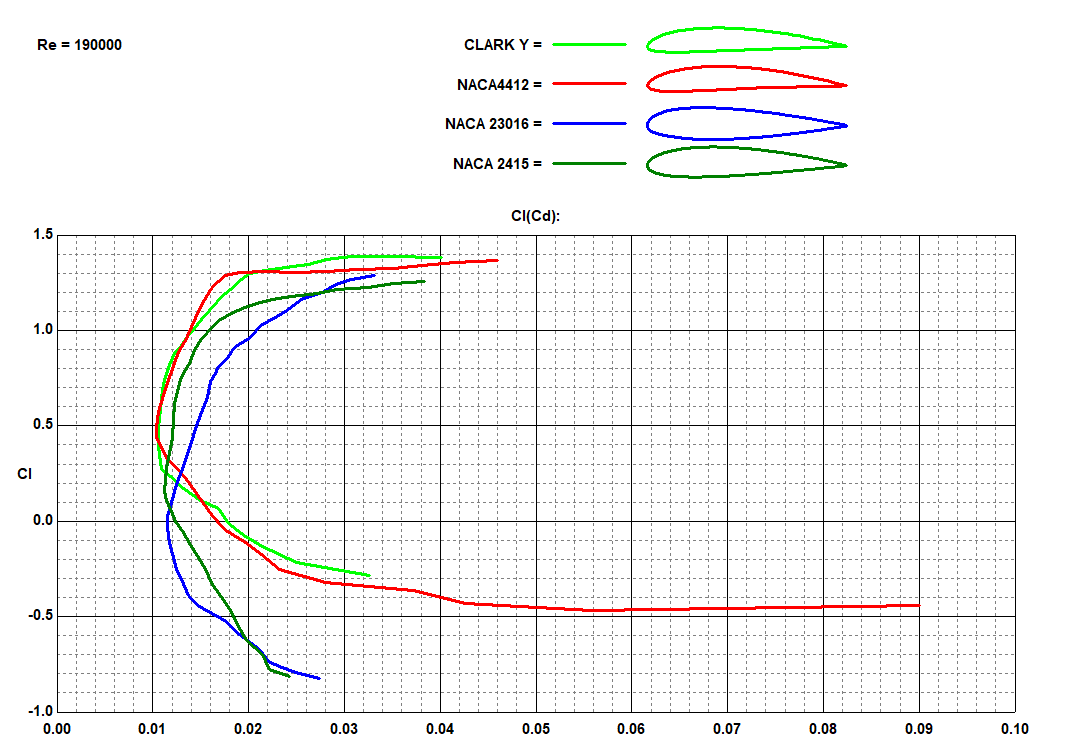
\includegraphics[width=0.5\columnwidth]{四种翼型的级曲线.png}
		\captionof{figure}{四种翼型的曲线}
	\end{center}
	\begin{center}
		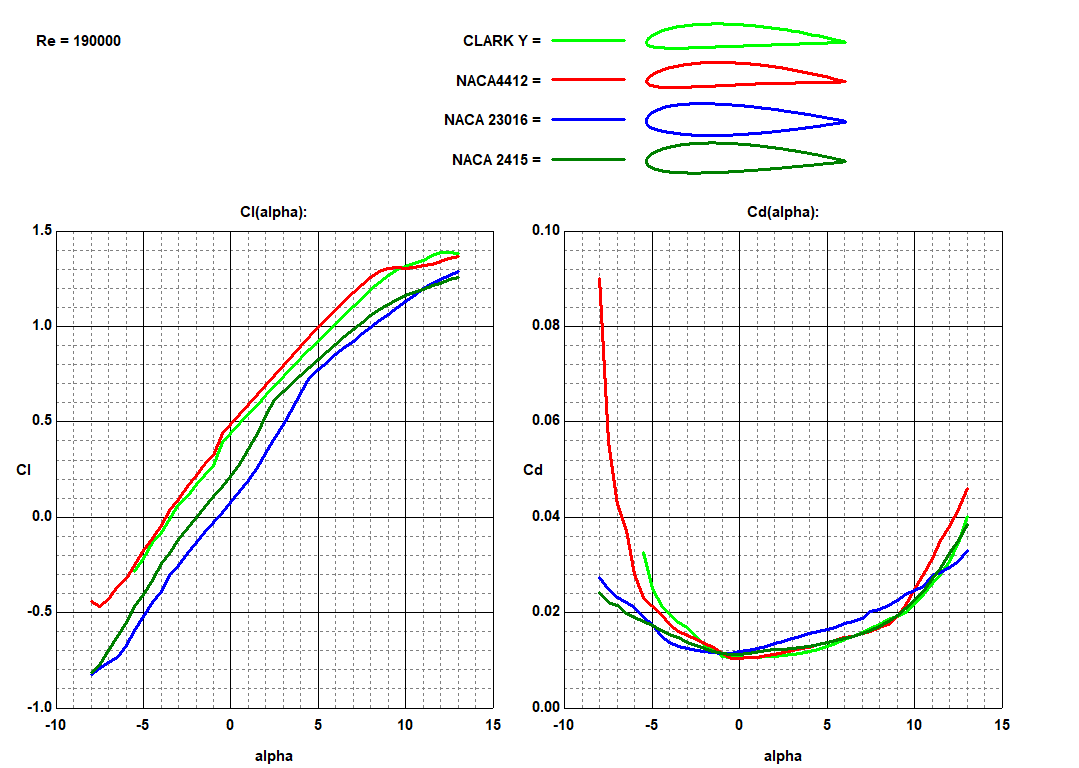
\includegraphics[width=0.5\columnwidth]{升阻力系数与攻角关系图.png}
		\captionof{figure}{升阻力系数与攻角关系图}
	\end{center}
	\begin{center}
		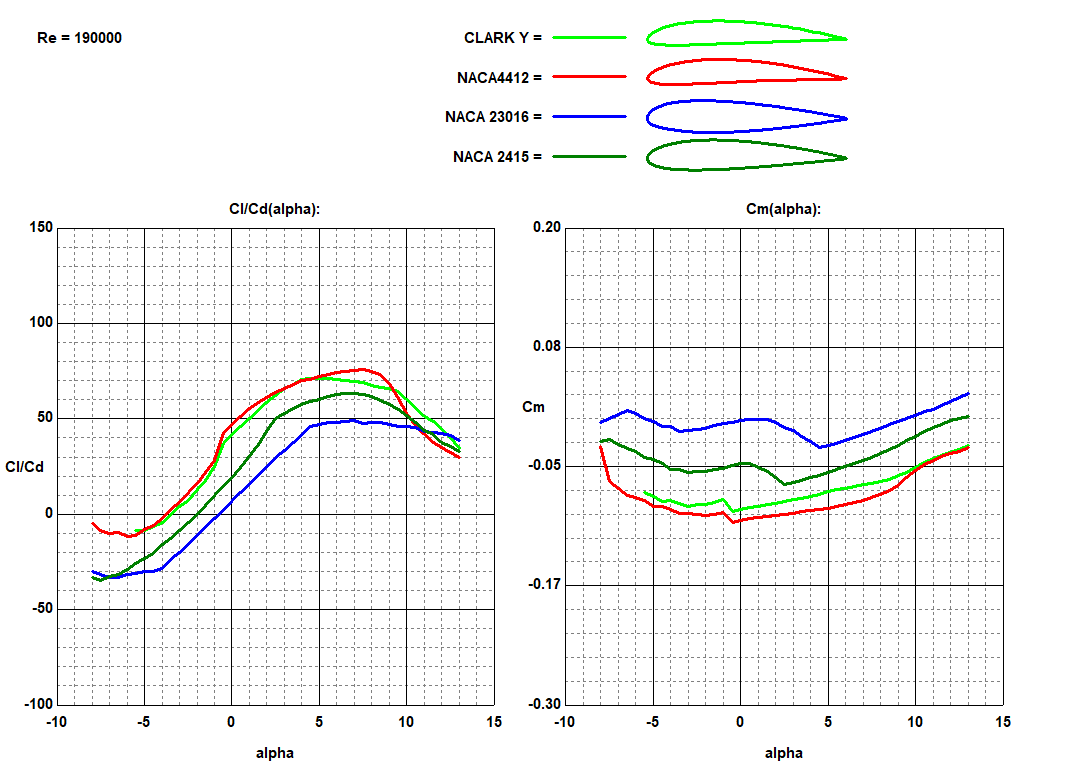
\includegraphics[width=0.5\columnwidth]{升阻比,俯仰力矩系数随攻角的变化.png}
		\captionof{figure}{升阻比,俯仰力矩系数随攻角的变化}
	\end{center}
	综合以上三图，考虑到升力系数最大需要达到1.6以上，因此可以选择NACA4412、CLARK-Y两种翼型。考虑到NACA-4412与CLARK-Y两种翼型之间在不同参数下都比较接近，仅在俯仰力矩系数处有8\%左右的差别。考虑到CLARK-Y翼型为上弯下平的简单几何，制造和手工修型非常容易；而NACA4412为上下表面均弯曲的翼型，轮廓复杂，制造精度要求高，通常需要数控切割或精密模具。所以最终主机翼与水平尾翼选择CLARK-Y翼型
	
	尾翼翼型需要保持对称，目前比较常用的对称翼型为NACA 00系列的翼型，如NACA 0006，NACA0008，NACA0009，NACA0012，NACA0015，同理绘制几种翼型的相关曲线图如下
	\begin{center}
		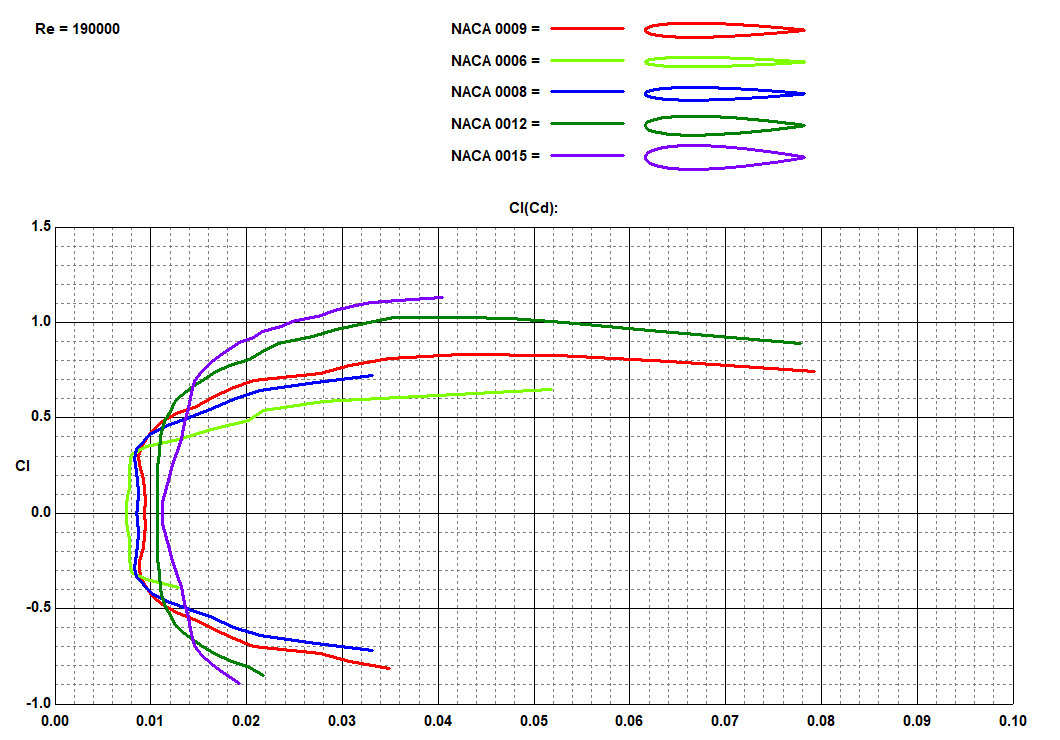
\includegraphics[width=0.5\columnwidth]{垂尾五种翼型的极曲线.png}
		\captionof{figure}{五种翼型的曲线}
	\end{center}
	\begin{center}
		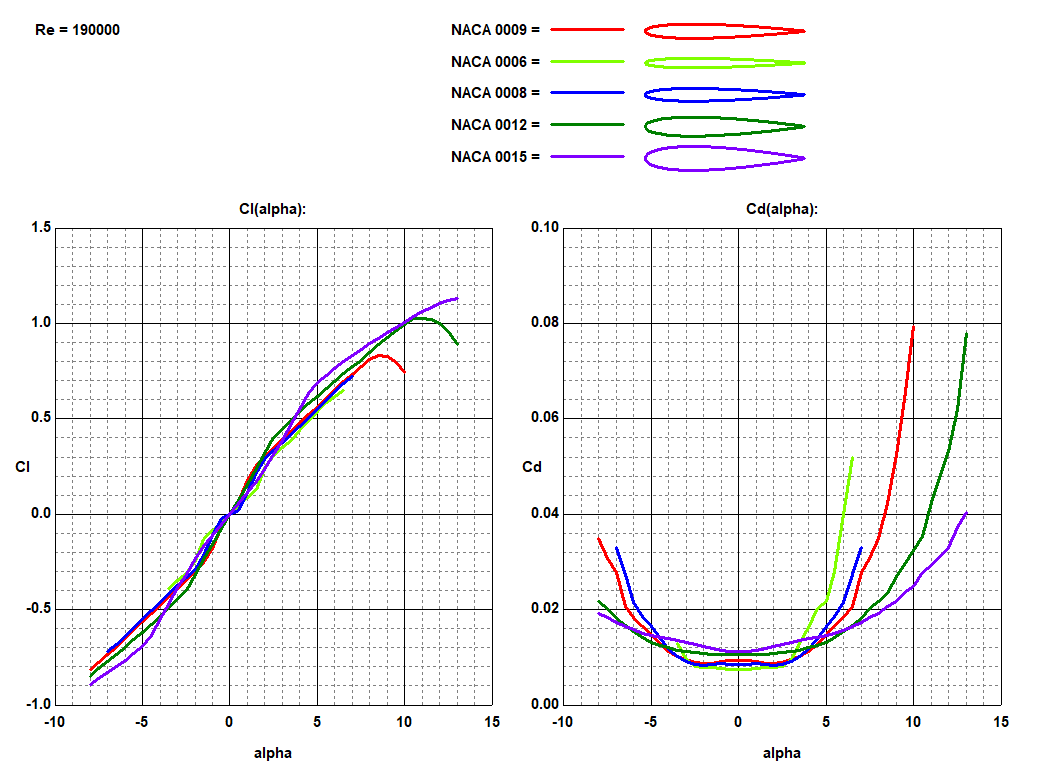
\includegraphics[width=0.5\columnwidth]{垂尾五种翼型升阻力系数随攻角关系图.png}
		\captionof{figure}{升阻力系数与攻角关系图}
	\end{center}
	\begin{center}
		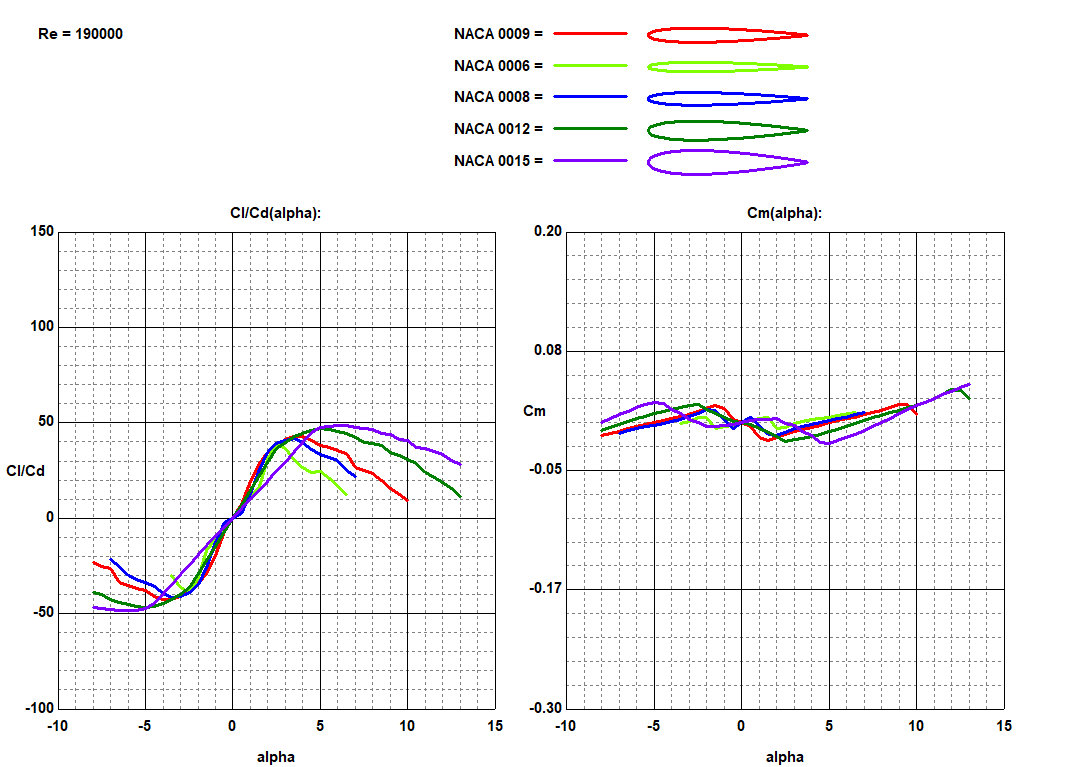
\includegraphics[width=0.5\columnwidth]{垂尾五种翼型的升阻比，俯仰力矩系数随攻角的变化.png}
		\captionof{figure}{升阻比,俯仰力矩系数随攻角的变化}
	\end{center}
	不难发现这几种翼型相差不大，同时考虑到垂直尾翼一要有足够的厚度为翼梁和蒙皮提供空间，从而轻松应对飞行中的气动载荷和地面操作的轻微碰撞，二则不应当显著增加重量和惯性。所以我们采用NACA0009这样中庸的选择。
	
	\subsubsection{质心位置的估算}
	通过跑飞机的Xflr5仿真可以得到以下的数据，其中
	\[XNP=352.089\]
	其中其坐标原点的选取为机头处，X轴方向向机尾，取在机身中轴线上\\
	所以飞机的静稳定裕度取值在$5\%-15\%$范围内，得到下列质心位置参考表格
	\begin{center}
		\captionof{table}{不同静稳定裕度对应的质心位置}
		\label{tab:cg_position}
		\begin{tabular}{S[table-format=2.0] S[table-format=1.2] S[table-format=4.4] S[table-format=6.4]}
			\toprule
			{\begin{tabular}[c]{@{}c@{}}静稳定裕度\\ (\% MAC)\end{tabular}} & 
			{$k$} & 
			{$k \times \rm MAC$ (\unit{\milli\meter})} & 
			{质心位置 $CG$ (\unit{\milli\meter})} \\
			\midrule
			5  & 0.05 & 7.7243 & 343.5977 \\
			6  & 0.06 & 9.2692 & 342.0528 \\
			7  & 0.07 & 10.8140 & 340.5080 \\
			8  & 0.08 & 12.3589 & 338.9631 \\
			9  & 0.09 & 13.9037 & 337.4183 \\
			10 & 0.10 & 15.4486 & 335.8734 \\
			11 & 0.11 & 16.9935 & 334.3285 \\
			12 & 0.12 & 18.5383 & 332.7837 \\
			13 & 0.13 & 20.0832 & 331.2388 \\
			14 & 0.14 & 21.6280 & 329.6940 \\
			15 & 0.15 & 23.1729 & 328.1491 \\
			\bottomrule
		\end{tabular}
	\end{center}
	这里取中值，也即静稳定裕度在10\%时的位置作为质心位置
	\[X_C=335.8734\,\mathrm{mm}\]
	\subsection{气动特性分析}
	\subsubsection{飞机纵向气动分析}
	下面给出在不包含机体的情况下运行XFLR5得到的静稳定性分析，在100 m高度仿真
	\begin{center}
		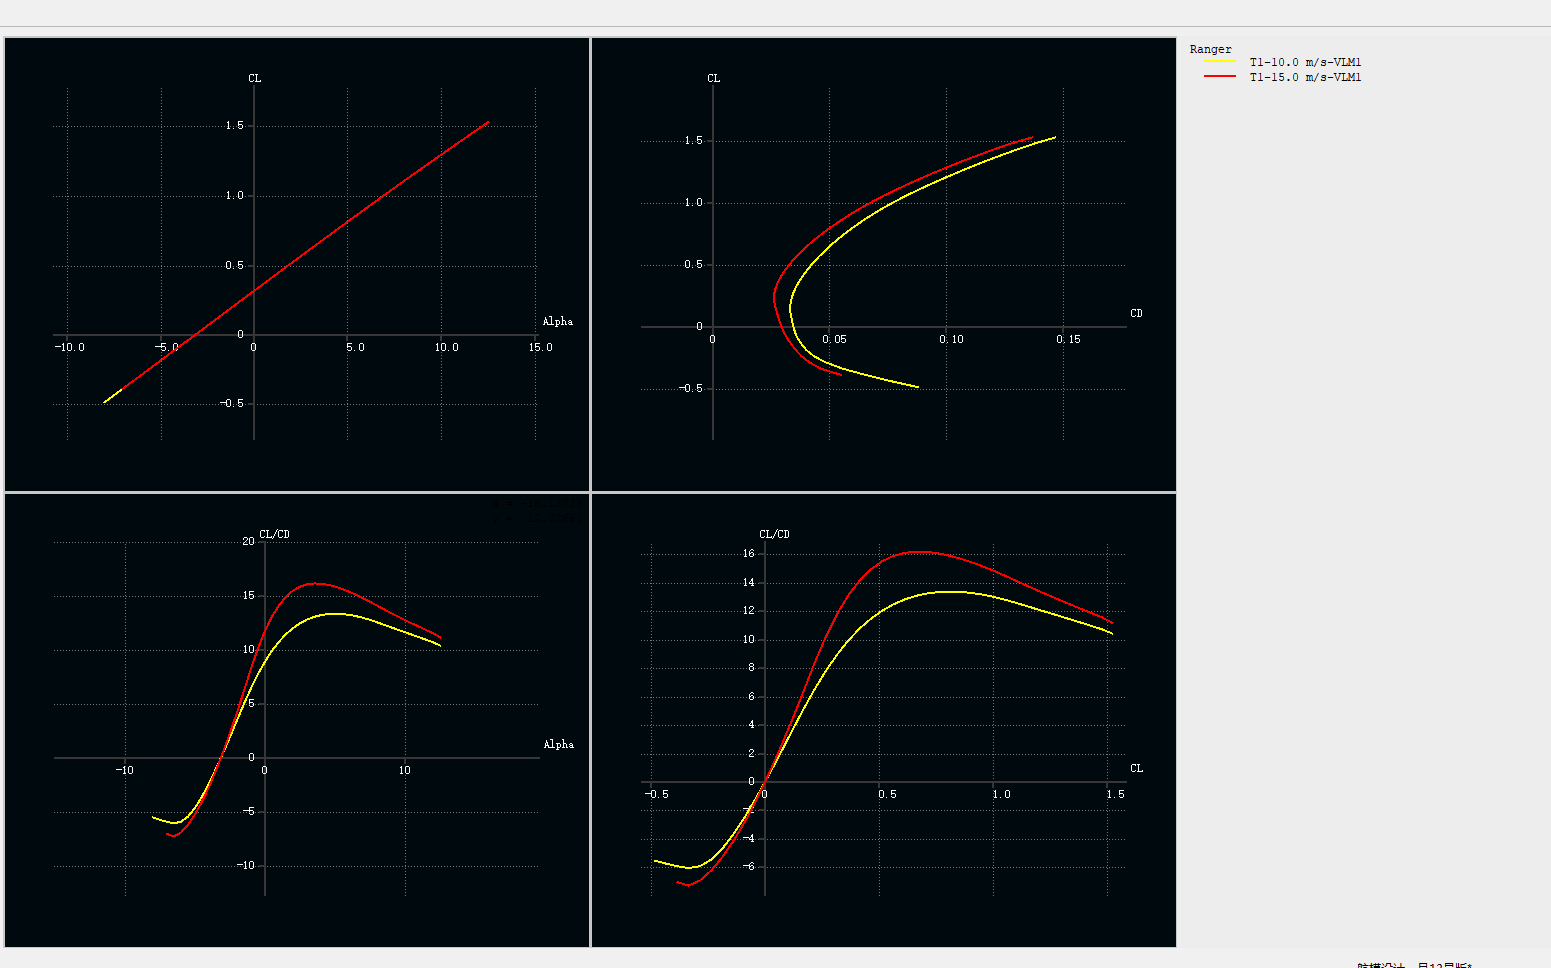
\includegraphics[width=0.5\columnwidth]{前四张图.png}
		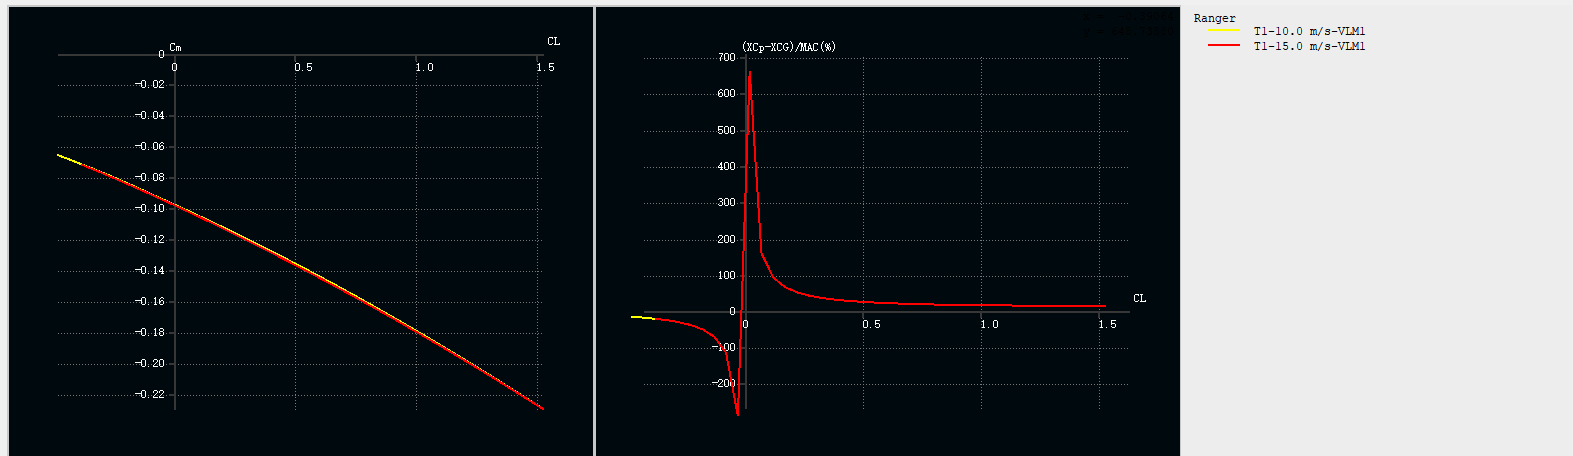
\includegraphics[width=0.5\columnwidth]{后面两张图.png}
		\captionof{figure}{全机纵向气动特性曲线}
	\end{center}
	\begin{enumerate}
		\item 零升迎角约-3°，升力线斜率0.096/°，巡航升力系数（CL=0.6）对应迎角约4.0°，失速迎角大于15°，失速发展和缓；
		\item 在巡航速度15 m/s下，全机最大升阻比超过15.0，对应升力系数约0.6，接近巡航升力系数；高升阻比范围较宽，便于高效率飞行；
		\item 俯仰力矩系数表明，无人机在计算攻角范围内具有纵向稳定性，攻角越大，稳定性越强。
		\item 巡航点附近纵向稳定裕度约-22\%(MAC)，随攻角增大，稳定裕度变化较小。无人机的抗失速能力较好，不易进入大攻角状态。
	\end{enumerate}
	
	\section{飞行性能初步评估}
	
	根据设计参数和气动分析结果，对该无人机的各项飞行性能进行评估如下：
	
	\subsection{定常直线水平运动性能}
	
	在定常直线水平飞行中，升力等于重力，推力等于阻力。
	
	\begin{itemize}
		\item \textbf{巡航状态}（高度100 m，速度15 m/s）：
		\begin{itemize}
			\begin{spacing}{0.8}
				\item 升力系数：$C_L \approx 0.6$
				\item 阻力系数：$C_D \approx 0.0433$
				\item 所需推力：$T \approx 0.93 \, \text{N}$
				\item 所需功率：$P \approx 14 \, \text{W}$
			\end{spacing}
		\end{itemize}
		
		\item \textbf{平衡方程}：
		\[
		L = W = \frac{1}{2} \rho V^2 S C_L, \quad T = D = \frac{1}{2} \rho V^2 S C_D
		\]
		其中：$W = mg = 1.3 \times 9.8 = 12.74 \, \text{N}$，$S = 0.1576 \, \text{m}^2$，$\rho = 1.213 \, \text{kg/m}^3$。
	\end{itemize}
	
	\subsection{平飞飞行性能}
	
	\begin{itemize}
		\begin{spacing}{0.8}
			\item \textbf{最小平飞速度}：
			\begin{itemize}
				\item 无襟翼（$C_{L\max} = 1.2$）：$V_{\min} = \sqrt{\frac{2W}{\rho S C_{L\max}}} \approx 10.55 \, \text{m/s}$
				\item 着陆襟翼下偏35°（$C_{L\max} = 1.698$）：$V_{\min} \approx 8.87 \, \text{m/s}$
			\end{itemize}
			
			\item \textbf{最大平飞速度}（受推力限制，假设最大推力 $T_{\max} = 6.37 \, \text{N}$）：
			由极速约束方程求解：
			\[
			\frac{T_{\max}}{mg} = C_{\mathrm{D0}}\frac{\rho V^2}{2g}\left(\frac{m}{S}\right)^{-1} + \frac{1}{\pi Ae}\frac{2g}{\rho V^2}\left(\frac{m}{S}\right)
			\]
			代入参数解得理论最大速度约 $47 \, \text{m/s}$，但实际电动机推力随速度增加而下降，保守估计最大平飞速度约 $20 \, \text{m/s}$。
			
			\item \textbf{速度范围}：$8.87 \, \text{m/s} \leq V \leq 20 \, \text{m/s}$（实际使用中可能限制在15 m/s以内）。
		\end{spacing}
	\end{itemize}
	
	\subsection{上升性能}
	
	假设发动机最大推力 $T_{\max} = 6.37 \, \text{N}$ 且不随速度变化（简化模型）。
	
	\begin{itemize}
		\begin{spacing}{0.8}
			\item \textbf{剩余推力}：$\Delta T = T_{\max} - D$
			
			\item \textbf{上升率}：$V_v = \frac{\Delta T \cdot V}{W}$
			
			\item \textbf{最大上升率}：约 $8.8 \, \text{m/s}$，出现在速度 $25 \sim 30 \, \text{m/s}$ 区间，但该速度可能超出电动机高效工作范围。
			
			\item \textbf{实用上升率}（巡航速度15 m/s）：约 $6.4 \, \text{m/s}$。
			
			\item \textbf{最大上升角}：$\theta_{\max} = \arcsin\left(\frac{\Delta T_{\max}}{W}\right)$，在失速速度附近约 $25.5^\circ$，对应速度 $10.55 \, \text{m/s}$。
		\end{spacing}
	\end{itemize}
	
	\subsection{下降性能}
	
	\begin{itemize}
		\begin{spacing}{0.8}
			\item \textbf{滑翔比}：最大升阻比 $K_{\max} \approx 15$，对应速度 $12.16 \, \text{m/s}$。
			
			\item \textbf{最小下降率}：约 $0.81 \, \text{m/s}$，对应下降角 $3.81^\circ$。
			
			\item \textbf{无动力滑翔距离}：从100 m高度可滑翔约 $1500 \, \text{m}$（理想条件）。
			
			\item \textbf{下降率方程}：
			\[
			V_v = V \cdot \sin\gamma = V \cdot \frac{D}{L} = \frac{V}{K}
			\]
		\end{spacing}
	\end{itemize}
	
	\subsection{机动性能}
	
	\begin{itemize}
		\begin{spacing}{0.8}
			\item \textbf{最大过载}（巡航速度15 m/s，$C_{L\max} = 1.2$）：
			\[
			n_{\max} = \frac{\rho V^2 S C_{L\max}}{2W} \approx 2.02
			\]
			
			\item \textbf{最小盘旋半径}（15 m/s，最大过载）：
			\[
			r_{\min} = \frac{V^2}{g \sqrt{n_{\max}^2 - 1}} \approx 13.1 \, \text{m}
			\]
			
			\item \textbf{盘旋角速度}：
			\[
			\omega_{\max} = \frac{g\sqrt{n_{\max}^2 - 1}}{V} \approx 1.15 \, \text{rad/s} \approx 65.9^\circ/\text{s}
			\]
			
			\item \textbf{滚转性能}：副翼最大偏转角 $\pm 25^\circ$，可提供足够的滚转控制力矩。
		\end{spacing}
	\end{itemize}
	
	\subsection{起降性能}
	
	\begin{itemize}
		\begin{spacing}{0.8}
			\item \textbf{起飞距离}（无襟翼，最大推力6.37 N）：
			\[
			x_{\mathrm{T.O.}} = \frac{m^2 k_{\mathrm{T.O.}}^2 g}{F \rho S C_{L\max}} \approx 19.6 \, \text{m}
			\]
			使用起飞襟翼（下偏12°）可进一步缩短。
			
			\item \textbf{着陆滑跑距离}（襟翼下偏35°，摩擦系数 $\mu = 0.2$）：
			\[
			x_{\mathrm{LGR}} = \frac{k_{\mathrm{T.D.}}^2 m}{\mu \rho S C_{L\max}} \approx 33.8 \, \text{m}
			\]
			
			\item \textbf{起降跑道要求}：远低于100 m，具备良好的短距起降（STOL）能力。
			
			\item \textbf{起降速度}：
			\begin{itemize}
				\item 起飞离地速度：$V_{\mathrm{T.O.}} = k_{\mathrm{T.O.}} \sqrt{\frac{2mg}{\rho S C_{L\max}}} \approx 12.66 \, \text{m/s}$
				\item 着陆接地速度：$V_{\mathrm{T.D.}} = k_{\mathrm{T.D.}} \sqrt{\frac{2mg}{\rho S C_{L\max}}} \approx 11.42 \, \text{m/s}$
			\end{itemize}
		\end{spacing}
	\end{itemize}
	
	\subsection{总结}
	
	该无人机设计满足最大总重1.3kg的基本任务需求，并具备以下性能特点：
	
	\begin{enumerate}
		\begin{spacing}{0.8}
			\item \textbf{良好的低速性能}：失速速度低至8.87 m/s（襟翼展开），起降安全余量充足。
			\item \textbf{高效的巡航效率}：最大升阻比达15，巡航功耗低。
			\item \textbf{出色的短距起降能力}：起飞距离<20 m，着陆滑跑距离<34 m，适应简易跑道。
			\item \textbf{足够的机动性}：最大过载2.02，可完成协调转弯等基本机动。
			\item \textbf{稳定的下降滑翔}：滑翔比高，紧急情况下可无动力安全着陆。
		\end{spacing}
	\end{enumerate}
	
	\textbf{注}：部分性能（如最大速度、上升率）基于推力恒定假设，实际性能需根据选定的电动机和螺旋桨特性曲线进一步验证。总体而言，该设计在气动效率和任务适应性之间取得了良好平衡。
\end{document}

%给cx的小建议
%下标要严格区分正体和斜体。有实际意义则用正体，若只是一个指标则用斜体。
%所有单位用正体，并且最好和数值之间留一点空格
%角度不应该用字母o表示，有圆圈的命令\circ
%你的最大起飞重量我取的1.3，你在最前面还有一个1.5的值，一定要统一一遍。 完成


%<!--你知道q,K_1,K_2,D_D0是什么意思吗-->看文档后面有给定义，先写在这里 好吧
%我还是自己独立算一次吧，里面太多数据没有来由，且看起来不太准确
%OK,那我先打公式，不带数据了
%我的意思是这个文档太防御性证明了（）真的看起来就是一坨shift，物理量不声明直接引入，后面也没有“其中某某等于某某”解释
%你猜他说什么：多翻翻手册，救赎之道就在其中啊 ？？？什么手册 对不起，我是sb
%好像他说的就是我之前发给你的那个
%是那本书吗？z-lib的那本？是的 服了
%而且如果要细究，这个推导错误百出，第二个式子开头就掉了g，可信度大大的问号哈
%你说的对，那你用我上面给的机翼的详细数据算一下吧，机翼的数据还是对的
%还有个问题，就是他的文章是按照燃油机写的，很多技术性细节和我们的截然不同，方程也是很不一样。
%是的，所以我们最后不需要估计燃油重量
%发动机选型也不管